\documentclass[tikz, border=10pt]{standalone}
\usepackage{tikz}
\usetikzlibrary{decorations.pathmorphing, arrows.meta, shadings, calc, fadings}
\pagecolor{white}
\tikzfading[name=fade north, top color=transparent!100, bottom color=transparent!0]
\tikzset{
  atom/.style = {
    circle, shading=ball, ball color=black,
    minimum size = 32pt,
    text=white, font=\Large\bfseries\itshape,
    inner sep=0pt, outer sep=0pt
  },
  spr/.style = {
    decorate,
    decoration={coil, aspect=0.45, segment length=3.0mm, amplitude=4.5mm},
    gray!60, line width=2.0pt, line cap=round
  },
  bnd/.style  = {line width=3.5pt,  line cap=round, black!90},
  rarr/.style = {-{Stealth[length=7pt,width=5.5pt]},
                  red!90!black, line width=2.8pt},
  dbl/.style  = {{Stealth[length=7pt,width=5.5pt]}-{Stealth[length=7pt,width=5.5pt]},
                  red!90!black, line width=2.8pt}
}

\begin{document}
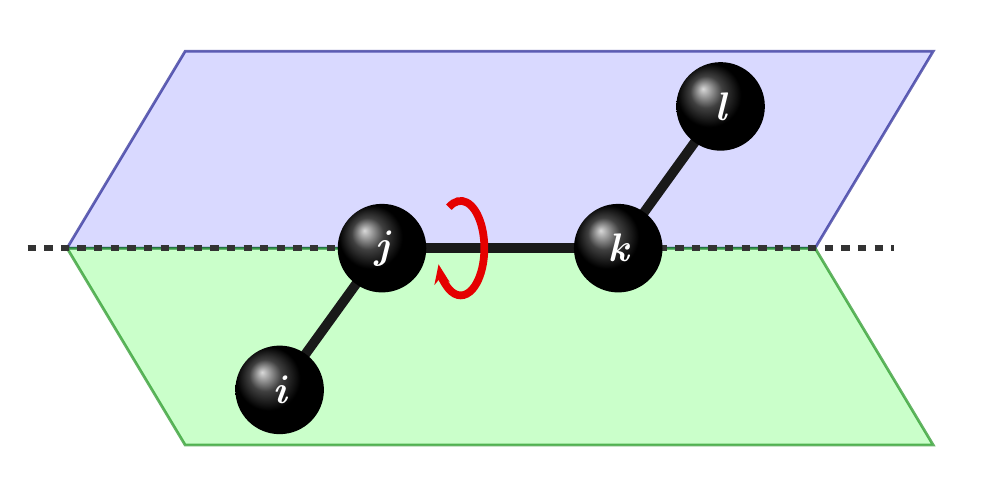
\begin{tikzpicture}[x=1cm, y=1cm]
  \useasboundingbox (-6.0, -2.8) rectangle (6.0, 2.8);
  %% Parallelogram bounds (Book fold)
  \coordinate (ML) at (-5.5,  0.0);
  \coordinate (MR) at ( 4.0,  0.0);
  
  \coordinate (TL) at (-4.0,  2.5);
  \coordinate (TR) at ( 5.5,  2.5);
  
  \coordinate (BL) at (-4.0, -2.5);
  \coordinate (BR) at ( 5.5, -2.5);

  %% Blue plane (top half)
  \fill[blue!25!white, opacity=0.6, draw=blue!50!black, line width=1pt]
    (ML) -- (MR) -- (TR) -- (TL) -- cycle;
    
  %% Green plane (bottom half)
  \fill[green!35!white, opacity=0.6, draw=green!50!black, line width=1pt]
    (ML) -- (MR) -- (BR) -- (BL) -- cycle;
    
  %% Dashed line
  \draw[dashed, line width=2pt, black!80] (-6.0, 0) -- (5.0, 0);

  %% Atoms positions
  \coordinate (Pj) at (-1.5,  0.0);
  \coordinate (Pk) at ( 1.5,  0.0);
  \coordinate (Pi) at (-2.8, -1.8);
  \coordinate (Pl) at ( 2.8,  1.8);

  %% Bonds
  \draw[bnd] (Pi) -- (Pj);
  \draw[bnd] (Pj) -- (Pk);
  \draw[bnd] (Pk) -- (Pl);

  %% Atoms
  \node[atom] (i) at (Pi) {\textit{i}};
  \node[atom] (j) at (Pj) {\textit{j}};
  \node[atom] (k) at (Pk) {\textit{k}};
  \node[atom] (l) at (Pl) {\textit{l}};

  %% Rotation arrow around j-k
  %% Draw a curved red arrow around the j-k bond
  \draw[rarr] (-0.5, 0) ++(120:0.3cm and 0.6cm) arc (120:-160:0.3cm and 0.6cm);


\end{tikzpicture}
\end{document}
